\section{Architecture and components}
\label{sec:arch}
The following chapter describes the individual components developed during this project as well as the interaction required between the components to fulfill the project goal of actuating the model car based on simulation data. A diagram that illustrates the interactions between the components is visible in \autoref{fig:arch}. \\

The data from the SpeedDreams simulation is first received by the mqtt server on the \texttt{car-control} topic, as described in \autoref{sec:mqtt-car-control}.
The component running on the PandaBoard is subscribed to this mqtt topic and processes the information, see \autoref{sec:panda}.
The resulting commands are then published on the \texttt{car-servo} mqtt topic, described in \autoref{sec:mqtt-car-servo}.
The component running on the Raspberry Pi (\autoref{sec:rpi}) in turn is responsible for forwarding the commands to the servo control component (\autoref{sec:servo}) according to the rules of the commands. \\

\begin{figure}[h]
    \centering
    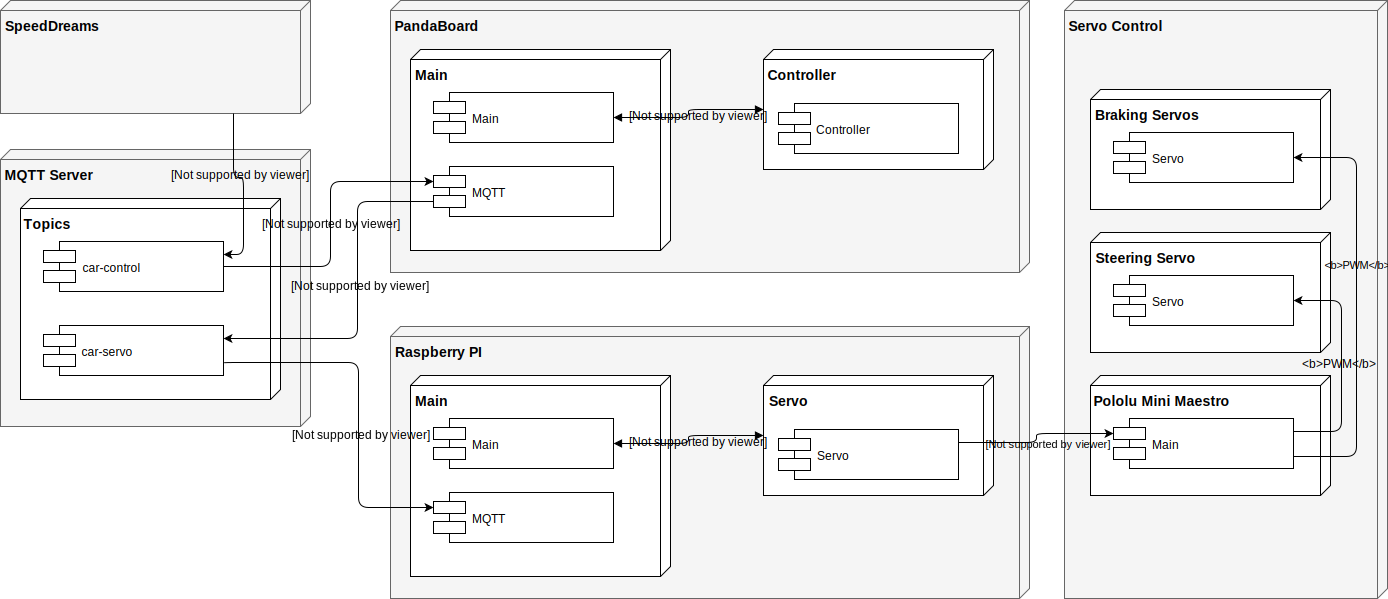
\includegraphics[width=1\linewidth]{images/components}
    \caption{Components overview}
    \label{fig:arch}
\end{figure}

\newpage

\subsection{Servo (CG)}
\label{sec:servo}
%TODO CG Write chapter
\subsection{Raspberry Pi (TM)}
\label{sec:rpi}
%TODO TM Write chapter
\subsection{PandaBoard}
\label{sec:panda}
%TODO FM: Write chapter
